\documentclass[11pt]{article}
\usepackage{lipsum,mathptmx,etoolbox}
\usepackage[american]{babel}
\usepackage[backend=biber, maxbibnames=100, style=ieee]{biblatex}
\renewcommand{\rmdefault}{phv} % Arial
\renewcommand{\sfdefault}{phv}
\usepackage{pgfgantt}
\usepackage{amsmath,amssymb}
\usepackage{xcolor}
\usepackage{booktabs}
\usepackage{pifont}
\usepackage[font={small}]{caption}
\usepackage{float}
\usepackage{xcolor}
\newcommand{\cmark}{\textcolor{green!60!black}{\ding{51}}}
\newcommand{\xmark}{\textcolor{red}{\ding{55}}}
\usepackage{tabularx}
\newcolumntype{Y}{>{\centering\arraybackslash}X}
\usepackage{csquotes}
\addbibresource{proposal.bib}
\usepackage{titlesec}
\titlespacing*\section{0pt}{-0pt plus 4pt minus 2pt}{0pt plus 2pt minus 2pt}
\titlespacing*\subsection{0pt}{-0pt plus 4pt minus 2pt}{0pt plus 2pt minus 2pt}
\titlespacing*\subsubsection{0pt}{-0pt plus 4pt minus 2pt}{0pt plus 2pt minus 2pt}
\setlength{\belowcaptionskip}{-15pt}
\setlength{\parindent}{.5cm}
\setlength{\parskip}{1.25ex}
\usepackage[
top    = 1.87cm,
bottom = 1.87cm,
left   = 1.27cm,
right  = 1.27cm]{geometry}
\usepackage{fancyhdr}
\pagestyle{fancy}
\renewcommand{\headrulewidth}{0pt}
\renewcommand{\footrulewidth}{0pt}
\lhead{}
\rhead{Talon Chandler}
\cfoot{}
\rfoot{\thepage}
\hyphenpenalty=1000
\begin{document}
\section*{Specific Aims}
Fluorescence microscopy is an extremely valuable tool in
biology---by introducing a fluorescent probe into a live organism and measuring
the position of the probe, researchers can watch cellular processes as they
occur. An extraordinary amount of effort has been expended towards improving the
spatial resolution of fluorescence microscopes, and recent breakthroughs have
allowed microscopes to achieve resolutions below the diffraction limit which has
enabled new biological insights \cite{nobel}.

Position is not the only property of fluorophores that can report on biological
processes, though. Early studies have shown that the \textit{orientation} of
fluorophores can report valuable information as well \cite{weiss1999}. Single
fluorophores that are attached to fixed structures absorb and emit light like
\textit{dipoles}---they absorb and emit polarized light anisotropically---so
their orientation can be measured using polarized light
microscopes. Unfortunately, current techniques can only measure the transverse
orientation of fluorophores in relatively thin specimens. These constraints
severely limit the number of biological questions that can be answered using
available orientation measurement techniques. In this work we propose the use of
polarized multiview microscopes to measure the three-dimensional orientation of
fluorophores in thick living specimens. We believe that this class of techniques
will enable new insights in structural and functional biology.

\noindent\textbf{Hypothesis:} Three-dimensional fluorescence orientation microscopy is a
valuable tool for investigating structural and functional biology in living
cells.

\noindent\textbf{Aim 1:} Develop a signal processing pipeline for analyzing and visualizing polarized multiview fluorescence microscopy data.

The raw data collected by polarized multiview fluorescence microscopes is not
easily interpreted in terms of fluorophore orientations. We propose a signal
processing pipeline that can efficiently reconstruct fluorophore orientations
from polarized multiview fluorescence microscopy data. An essential piece of
this pipeline is the spherical Fourier transform---by analyzing the data in the
angular frequency domain we can reconstruct fluorescence orientations much more
efficiently that existing techniques.

\noindent\textbf{Aim 2:} Demonstrate and verify three-dimensional fluorescence
orientation microscopy using a dual-view light-sheet microscope and a
light-field microscope.

We propose two complementary three-dimensional fluorescence orientation
microscopes---a dual-view light-sheet microscope and a light-field
microscope. The dual-view light-sheet microscope has isotropic spatial
resolution and a large field of view, but it suffers from long imaging times and
it delivers a large light dose to the sample. The light-sheet microscope has
complementary strengths and weaknesses---it images quickly and delivers a small
light dose, but it suffers from anisotropic spatial resolution and has a
relatively small field of view.

\noindent\textbf{Aim 3:} Demonstrate the value of three-dimensional fluorescence
orientation microscopy for live-cell biology.

Our overarching goal is to develop useful tools that will enable biological
discovery. To achieve this goal we will work directly with biologists who will
propose specific questions and experiments for the techniques we are
proposing. We expect that these interactions will inform and redirect our work
in ways that will improve the likelihood of biological discovery.

\pagebreak

\section*{Research Strategy}
\subsection*{Background}
A \textit{fluorescence microscope} is an optical imaging system that can measure
the position of fluorescent objects with a resolution of 1 $\mu$m or better.
Fluorescence microscopes excite fluorophores in a sample using short-wavelength
light and detect the long-wavelength light that the fluorophores emit as they
relax. By focusing the emitted light onto a plane detector using a series of
lenses, a fluorescence microscope creates a two-dimensional image of the
fluorophores in a sample.

Fluorescence microscopes image fluorescent samples, so how can we attain a
fluorescent sample? \textit{(1)~Find fluorescent samples in nature.} Most
organisms create fluorescent molecules naturally. Chlorophyll, collagen, and
melanin are examples of fluorescent molecules that are found in many plants and
animals. \textit{(2)~Add a fluorescent dye to a sample.}  There are hundreds of
commercially-available fluorescent dyes that can be introduced into a
sample. Researchers can choose a dye that will bind to a structure or process
that they are interested in studying.\hspace{0.4em}\textit{(3)~Genetically
  modify an organism so that it creates fluorescent proteins.} Many organisms
can be genetically modified so that a specific protein of interest displays
fluorescence. These techniques can be used to image almost any biological
process that involves proteins.

\begin{table}[b]
  \centering
  \begin{tabularx}{1\textwidth}{r *{4}{Y}}
    \toprule
&\multicolumn{2}{c}{Existing} &\multicolumn{2}{c}{Proposed} \\
\cmidrule(r){2-3} \cmidrule(r){4-5}
  & & Single- & Polarized &   \\
  Microscopy technique& Polarized single-view & molecule localization & dual-view light-sheet & Polarized light-field \\
  \midrule
Transverse spatial resolution & \cmark & \cmark\cmark\cmark & \cmark\cmark & \cmark \\
Axial spatial resolution & \xmark & \cmark\cmark\cmark & \cmark\cmark & \cmark \\
Transverse angular resolution & \cmark & \cmark & \cmark & \cmark \\
Axial angular resolution & \xmark & \cmark & \cmark & \cmark \\
Temporal resolution & \cmark & \xmark & \cmark & \cmark\cmark \\
Low dose & \cmark\cmark & \xmark & \cmark & \cmark\cmark \\
Inexpensive & \cmark\cmark & \cmark\cmark & \cmark & \cmark\cmark \\
Large field of view & \cmark & \cmark & \cmark\cmark & \cmark \\
\bottomrule
\end{tabularx}
  \caption{Comparison of existing and proposed fluorescence orientation microscopy techniques.}
\end{table}

Most fluorescence microscope models treat fluorophores as \textit{monopole
  absorbers} and \textit{monopole emitters}. These are valid approximations when
the fluorescent object contains many fluorophores that are rotating rapidly, but
in reality most fluorophores---including the widely used fluorophore, green
fluorescent protein (GFP)---behave like \textit{dipole absorbers} and
\textit{dipole emitters}. This is an important difference. Monopoles absorb and
emit all polarization states of light isotropically while dipoles absorb and
emit light in specific polarization states anisotropically. By sampling the
anisotropic absorption and emission patterns of a fluorophore we can estimate
the \textit{dipole axis} of the fluorophore. If the fluorophore is rigidly
attached to an oriented structure in a known way, then we can infer the
orientation of the structure from the estimated dipole axis.

Typical fluorescence microscopes are only capable of measuring the position of
fluorophores, but by adding \textit{polarizing filters} we can make a
fluorescence microscope sensitive to the anisotropic absorption and emission
patterns of fluorophores. If we place a polarizing filter in the excitation
light path, then the light that is incident on the sample is polarized and it
selectively excites fluorophores with dipole axes parallel to the light's
polarization. If we place a polarizing filter in the detection path, then we
selectively detect fluorophores with dipole axes parallel to the detected
polarization. By collecting images under several polarizing filter orientations
and applying a reconstruction scheme, we can estimate the position and
orientation of fluorophores in a sample.

\subsection*{Innovation}
Table 1 summarizes state-of-the-art techniques for measuring the orientation of
fluorophores. In this section we will briefly describe each technique and its
strengths and weaknesses. 

Polarized single-view microscopy \cite{demay2011} is the simplest fluorescence
orientation measurement technique. A simple single-view fluorescence microscope
can be modified into a polarized single-view microscope by adding a
liquid-crystal polarizing filter to the illumination or detection path. After
collecting intensity images under several polarizing filter orientations, the
orientation of fluorophores can be reconstructed by applying simple image
arithmetic to the set of images. Polarized single-view microscopes image quickly
and gently---many live-cell biology applications already use these
techniques---but they suffer from incomplete axial spatial and axial angular
resolution.

Single-molecule localization techniques do not require any special imaging
hardware---a plain fluorescence microscope can be used. Instead of special
hardware, a photo-activatable fluorophore is used so that the concentration of
excited fluorophores can be precisely controlled. By exciting and imaging
fluorophores one a time instead of all at once, the location and orientation of
the fluorophores can be determined extremely precisely. Although these techniques
can measure the position and orientation of fluorophores more precisely than any
other light-microscopy technique, they require extremely long imaging times and
large light doses. These constraints make localization techniques unsuitable for
many applications in biology where fast and gentle imaging are essential for
imaging live cells.

\begin{figure}[t]
\centering
\begin{minipage}{.45\textwidth}
  \centering
  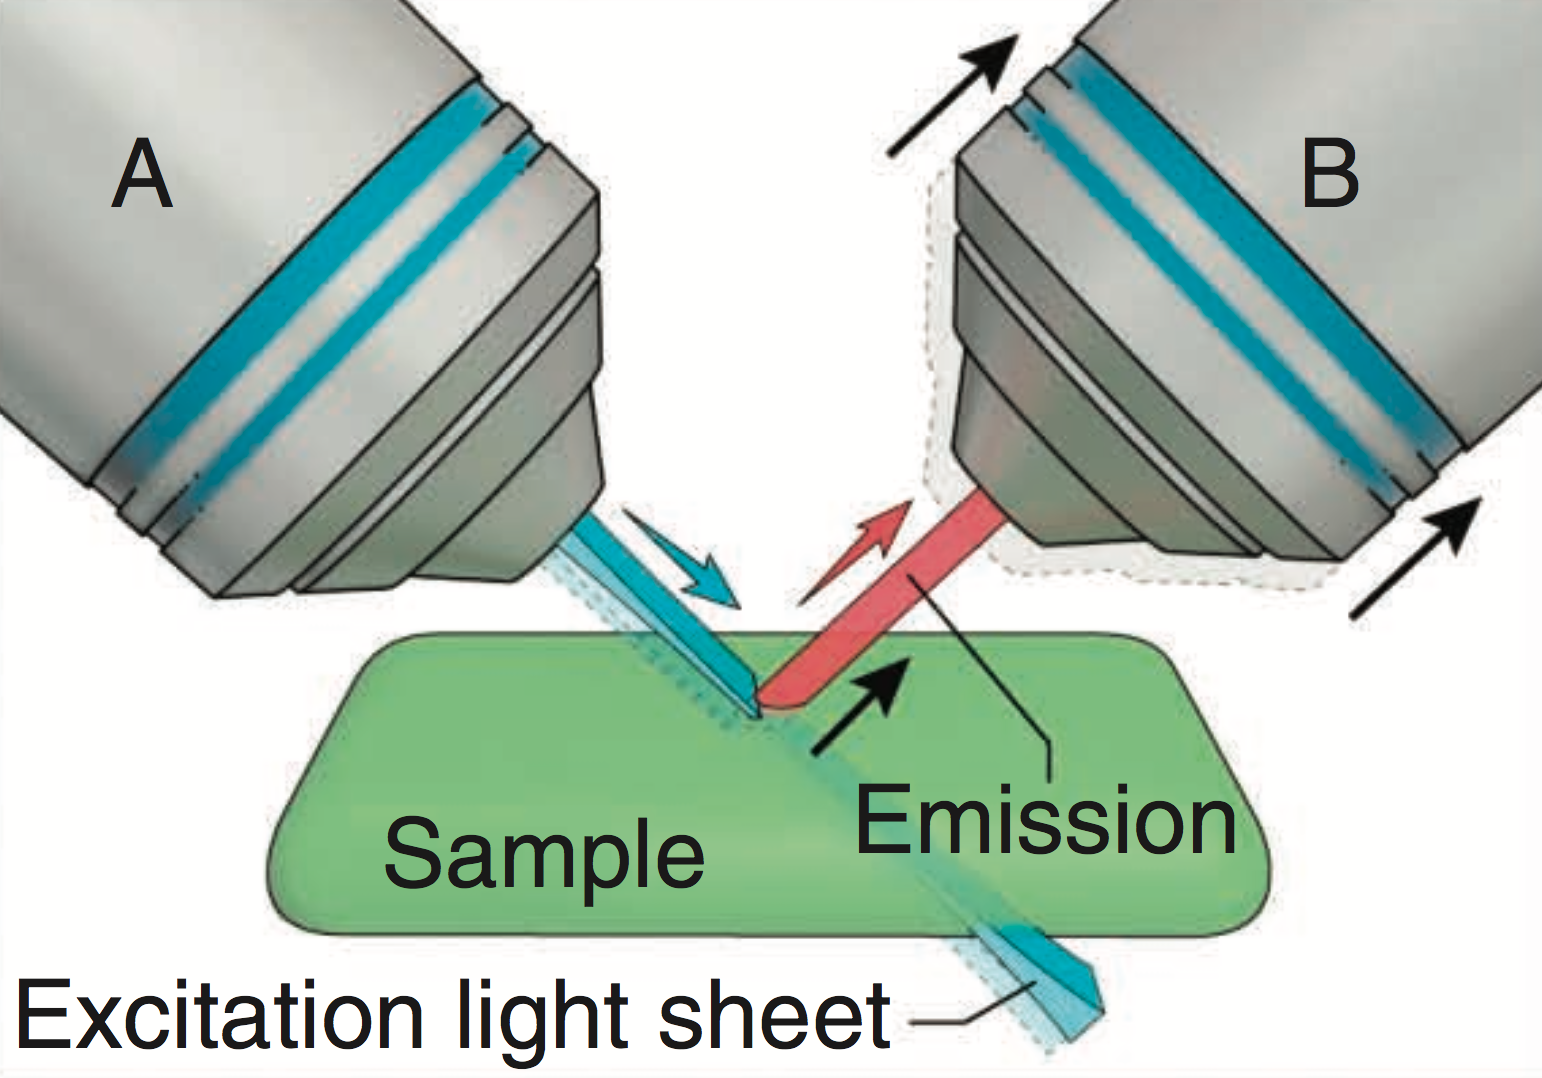
\includegraphics[width=\textwidth, interpolate=true]{figs/light-sheet}
  \caption{A dual-view light-sheet microscope excites the fluorophores in the
    sample with a light sheet originating from one objective, and it images the
    emitted light using the other objective as the light sheet sweeps through
    the sample. Next, the roles of the objectives are reversed and another set
    of images is acquired from the opposite view. We propose a dual-view
    light-sheet microscope outfitted with polarizing filters on each illumination
    arm. Figure from \cite{wu2013}.}
  \label{fig:dispim}
\end{minipage}%
\hspace{0.75em}
\begin{minipage}{.45\textwidth}
  \centering
  \vspace{-1.8em}
  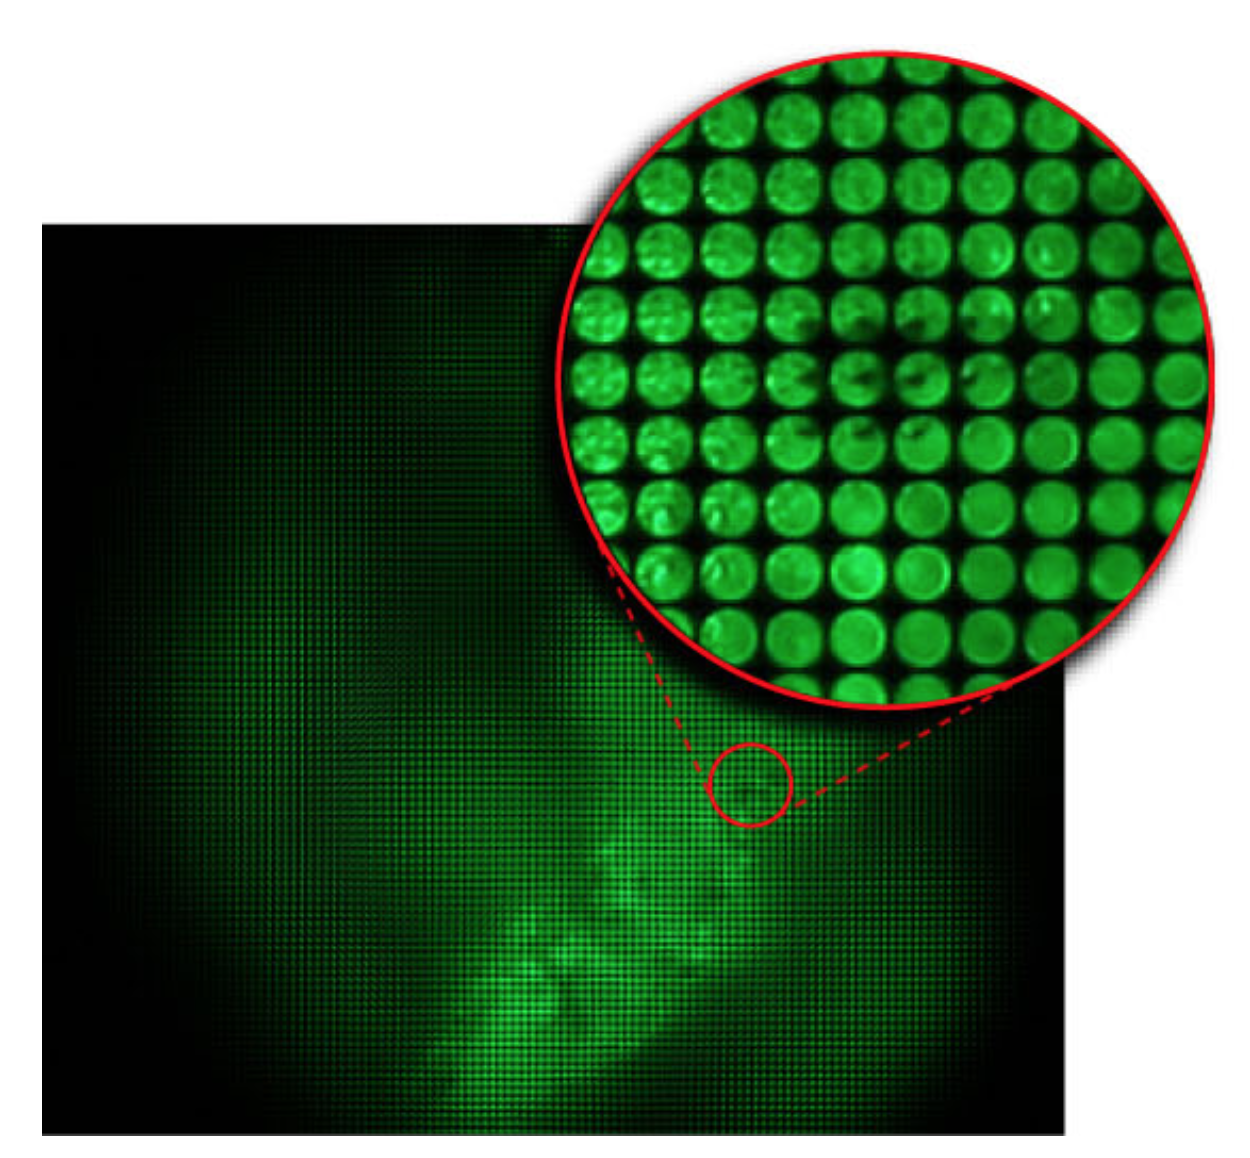
\includegraphics[width=\textwidth, interpolate=true]{figs/lf-fluo}
  \caption{A light-sheet microscope is an ordinary single-view microscope with a
    microlens array in the usual detector plane and the detector displaced to
    the focal plane of the microlenses. The image collected by a light-field
    microscope consists of many angular views of the sample collected at
    once. Figure from \cite{levoy2006}.}
  \label{fig:lf}
\end{minipage}
\end{figure}

Figure~\ref{fig:dispim} shows the imaging geometry for the proposed polarized dual-view
light-sheet microscope. This technique uses two objectives instead of one, and
it selectively excites planes of the sample to reduce phototoxicity. By using
the images from both views, this technique can achieve isotropic spatial
resolution, and it can measure the three-dimensional orientation of fluorophores
throughout a large field of view. Although this technique does not achieve the
high spatial resolution of single-molecule localization techniques, it can be
applied to large-volume live-cell imaging.

Figure~\ref{fig:lf} shows an image collected by a light-field microscope. By
replacing the usual detector plane with a microlens array and moving the
detector to the focal plane of the microlenses, a light-field microscope
captures many angular views of the sample at once. We can use these views and
limited-angle tomography reconstruction techniques to determine the
three-dimensional position of fluorophores throughout a sample. We propose the
addition of polarizing filters to the light-field microscope to measure the
three-dimensional orientation and position of the fluorophores. While the
proposed light-field approach has poorer resolution than the dual-view
light-sheet approach, the light-field approach is extremely fast and gentle, and
it will allow us to study fast-moving processes for long periods.

\subsection*{Preliminary Results}
\begin{figure}[t]
\centering
  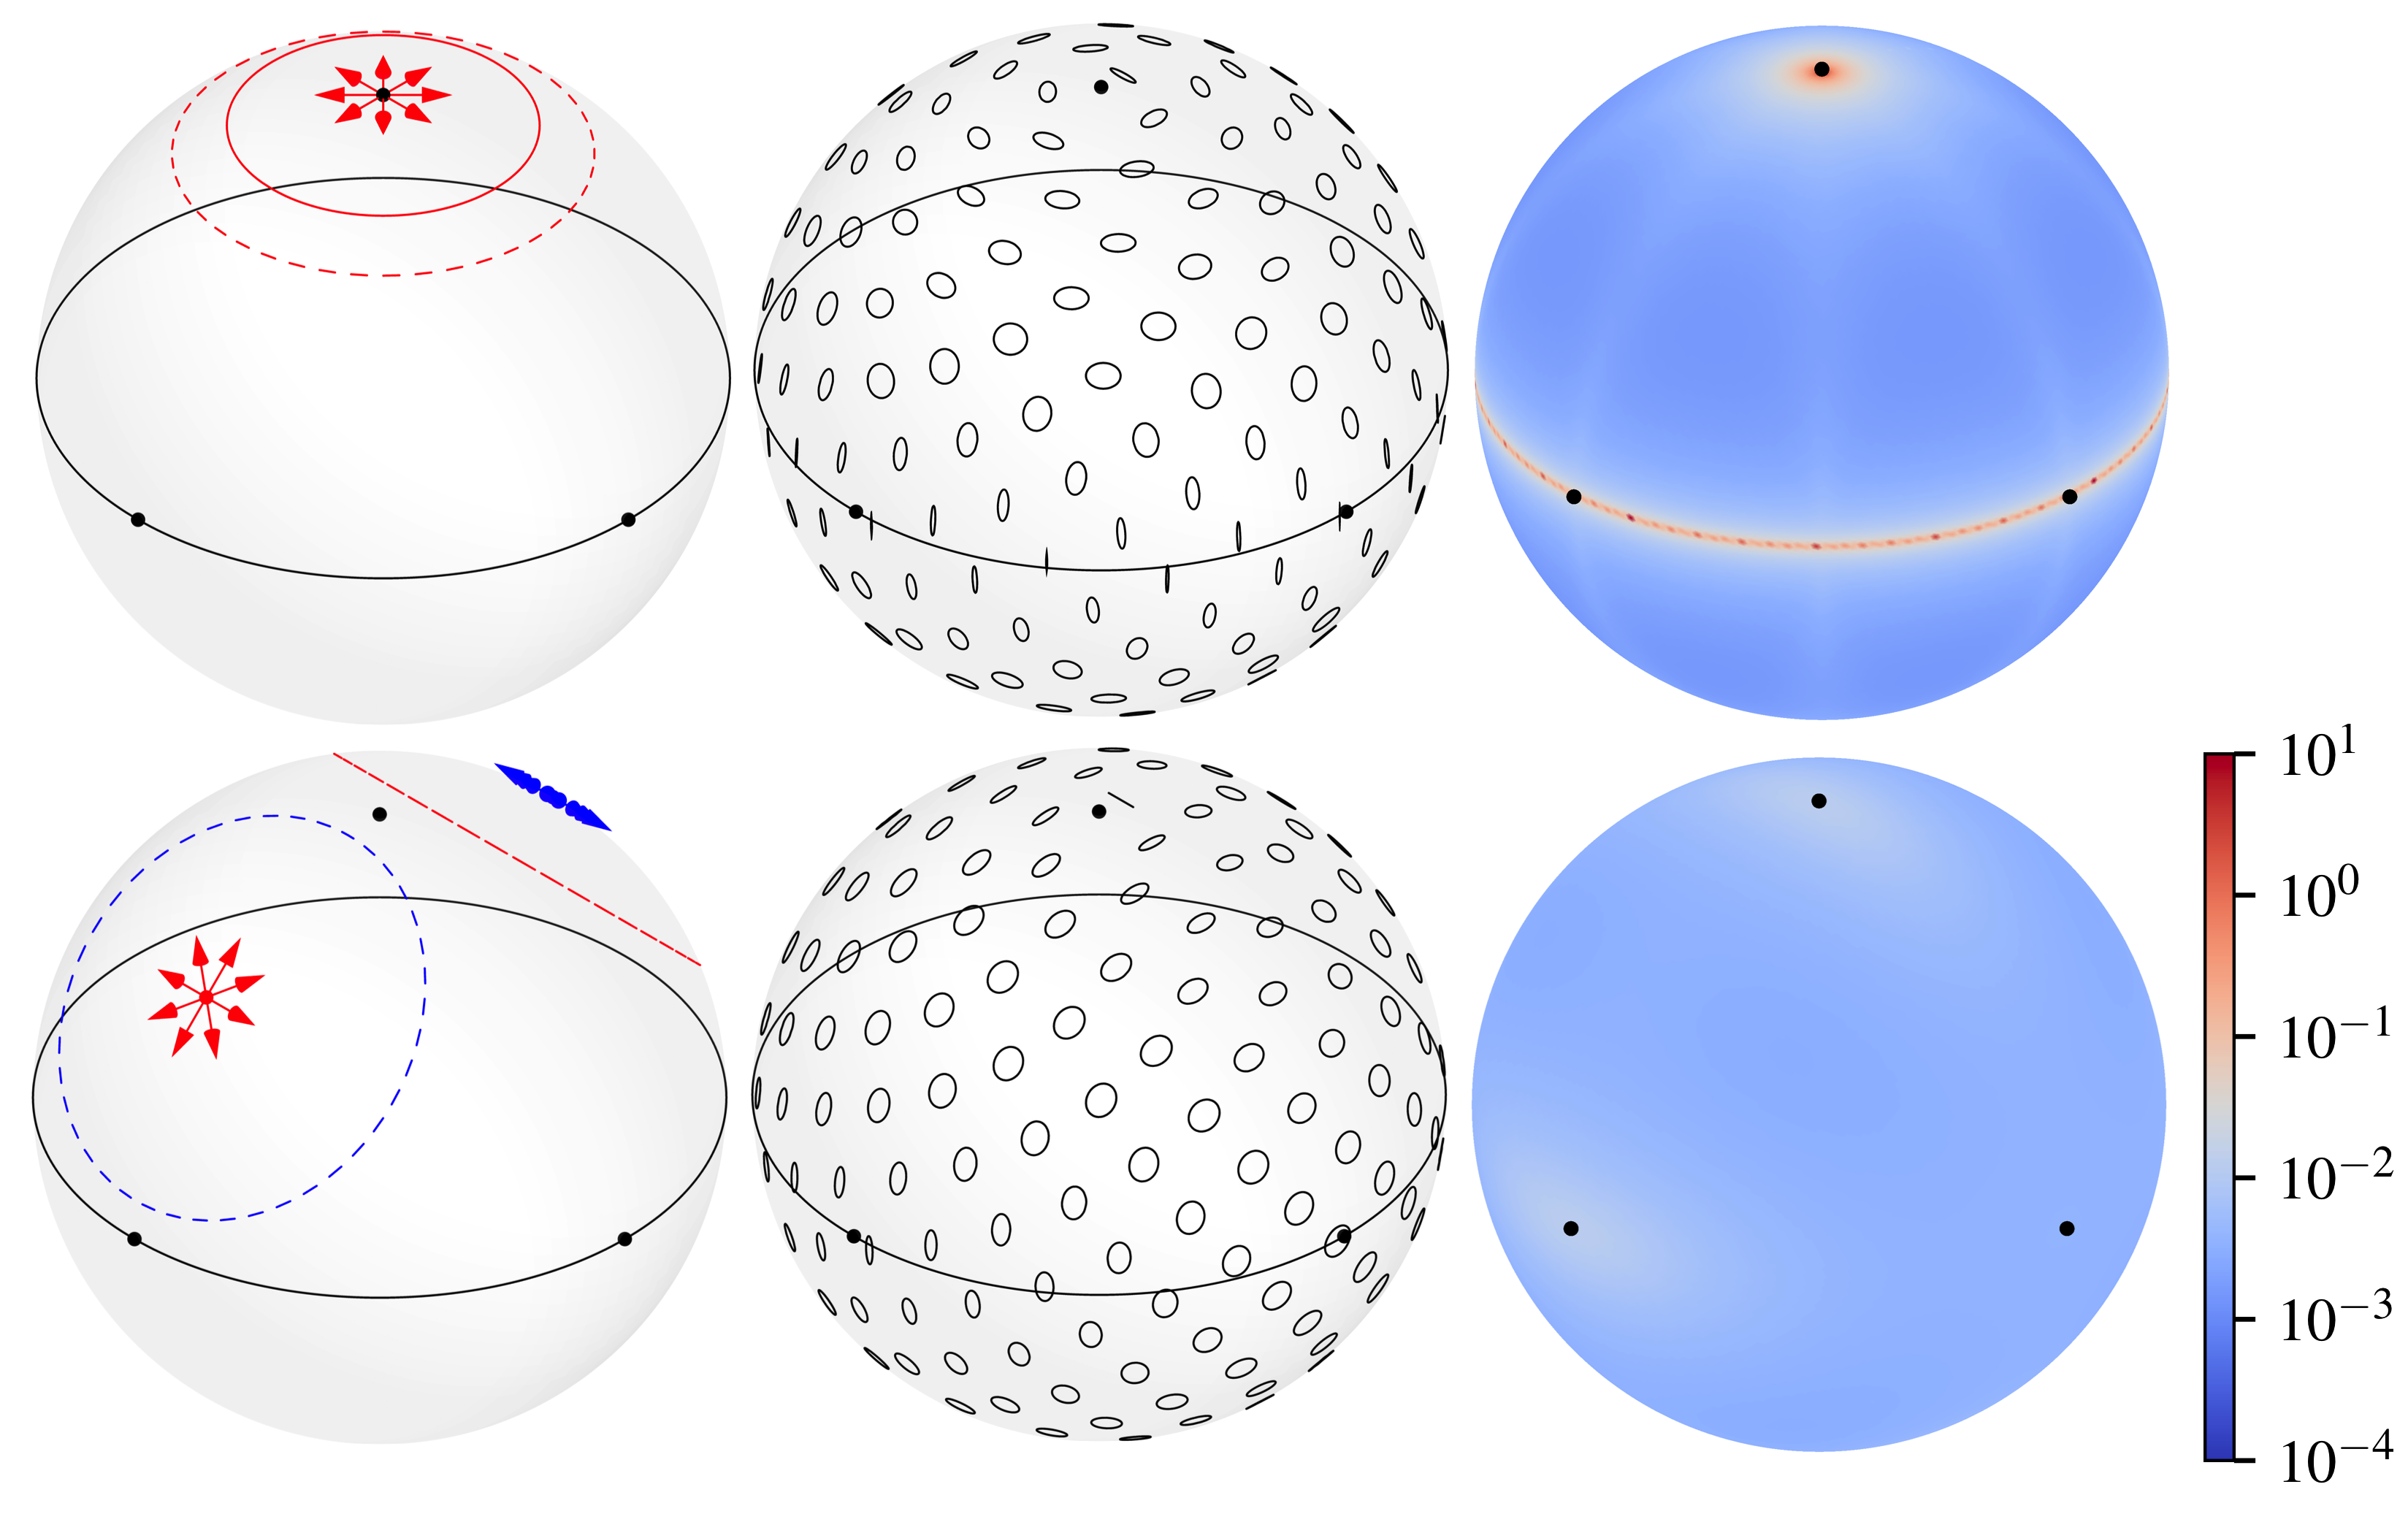
\includegraphics[width=0.8\textwidth, interpolate=true, trim={0em 0em 0em 0em}]{figs/proposal-fig}
  \caption{\textbf{Column 1:} Microscope schematics---arrows indicate polarized
    illumination orientations, solid lines indicate illumination NA, dashed
    lines indicate detection NA, and each color indicates a single illumination
    and detection path. \textbf{Column 2:} Uncertainty ellipses show the
    relative orientation uncertainty for single molecules along different
    directions. \textbf{Column 3:} The solid-angle uncertainty [sr] shows the
    absolute orientation uncertainty in all directions. All uncertainties are
    for the ideal case of a fixed single dipole---motion, homo-FRET, and higher
    order radiation moments will increase the true uncertainty. \textbf{Row 1:}
    0.8 NA single-view four-polarization epi-illumination
    microscope. \textbf{Row 2:} 0.8 NA orthogonal dual-view eight-polarization
    microscope. From columns 2 and 3 we can see that dual-view microscopes can
    estimate the orientation of fluorophores with fewer degeneracies and less
    uncertainty than single-view microscopes.}
  \label{fig:comparison}
\end{figure}
We have completed a theoretical study that investigates the limits of
orientation microscopy and the advantages of using multiple views
\cite{chandler17}. Figure~\ref{fig:comparison} shows our main result---dual-view
microscopes can measure the orientation of fluorophores with less fewer
degeneracies and less uncertainty than single-view microscopes. We also
developed a set of practical design heuristics that we will apply to the design
of our microscopes. In particular, we found that there is an optimal numerical
aperture for measuring the orientation of fluorophores---small apertures do not
collect enough photons and large apertures cannot distinguish between
fluorophores in different orientations. This result contradicts conventional
design wisdom in microscopy---increasing the numerical aperture improves
collection efficiency and spatial resolution, so conventional designers buy the
highest numerical aperture objective they can afford.

We have started to collect preliminary data with a polarized dual-view
light-sheet microscope. In our first study we imaged fixed cells stained with
Alexa Fluor 488 Phalloidin---a fluorescent dye that is known to attach parallel
to long actin fibers in the cells.  Figure~\ref{fig:recon} shows a prototype
three-dimensional orientation reconstruction using a simplified model applied to
real data. The results match our expectations---the reconstructed orientations
align with the long axes of the actin fibers.

Finally, we have collected preliminary images of several test specimens with
known fluorophore position and orientation including oriented fluorescent fibers
and giant unilamellar vesicles. These test specimens will be essential tools to
help us verify the results of our reconstructions.

\begin{figure}[t]
\centering
  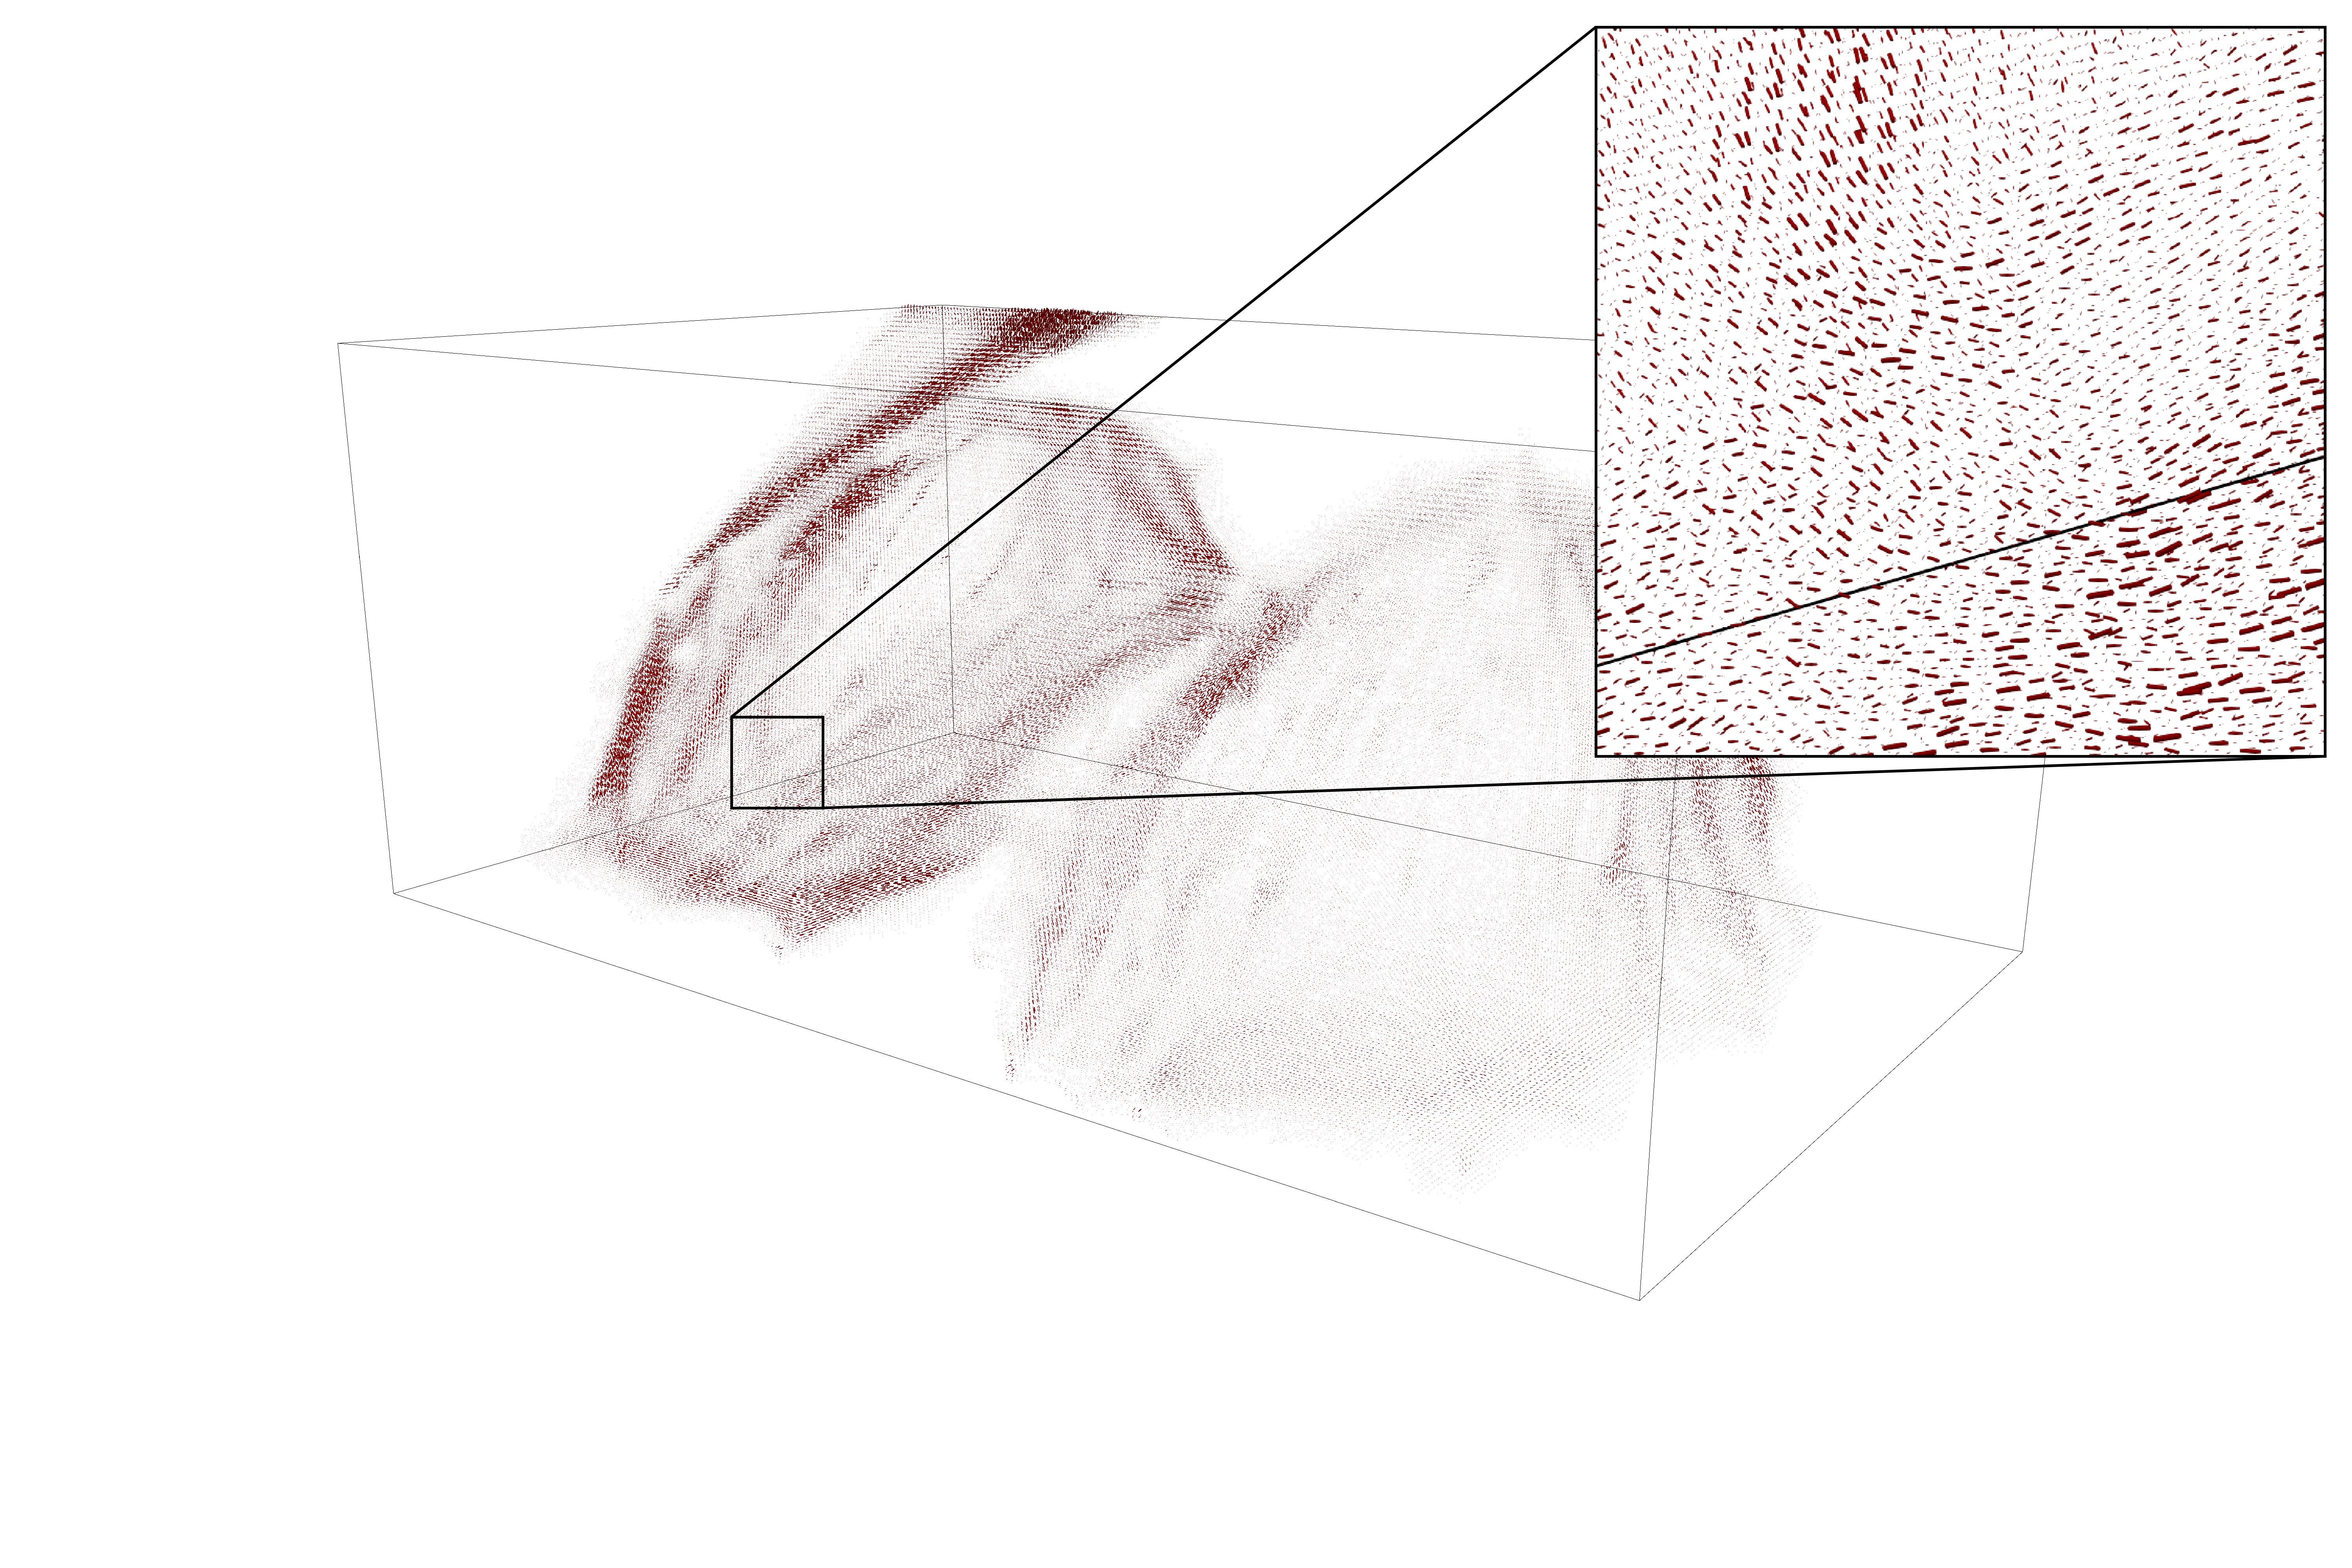
\includegraphics[width=0.65\textwidth, interpolate=true, trim={6em 4em 2em 0em}]{figs/inset}
  \caption{Orientation reconstruction of a 68$\times$108$\times$46 $\mu$m${}^3$
    volume of fixed cells stained with Alexa Fluor 488 Phalloidin and imaged
    with an asymmetric 1.1/0.71 NA dual-view light-sheet microscope. We assign a
    scaled and oriented glyph to each voxel to indicate the quantity and
    orientation of fluorophores in that voxel. The inset shows two crossed actin
    fibers, and our reconstructed orientations are aligned with the long axes of these
    fibers as expected.}
  \label{fig:recon}
\end{figure}


\subsection*{Approach}
\noindent\textbf{Aim 1:} Develop a signal processing pipeline for analyzing and
  visualizing polarized multiview fluorescence microscopy data.

  \noindent\textbf{Methods:} We will use physical modeling, linear systems
  theory, and optimization techniques to develop an efficient signal processing
  pipeline for the proposed microscopes. We have completed a prototype signal
  processing pipeline for reconstructing the three-dimensional orientation of
  fluorophores from polarized dual-view light-sheet microscope data, and we plan
  to improve this work by relaxing our assumptions and extending it to the
  light-field microscope.

  To illustrate our signal processing framework, consider a small voxel that
  contains many non-interacting fluorophores. We define the orientation
  distribution function $f(\hat{\mathbf{s}})$ as the number of fluorophores per
  steradian oriented in a direction $\hat{\mathbf{s}}$. The goal of polarized
  fluorescence microscopy is to estimate $f(\hat{\mathbf{s}})$ in many voxels
  throughout a three-dimensional sample.
  
  The forward model for an $N$-measurement polarized fluorescence microscope is
  given by
\begin{align}
  g_i = \int_{\mathbb{S}^2}d\hat{\mathbf{s}}\ h_i(\hat{\mathbf{s}})f(\hat{\mathbf{s}})\hspace{1em}\text{for}\hspace{1em} i=1,\dotsc,N,
\end{align}
where $h_i(\hat{\mathbf{s}})$ is the kernel of the $i$th microscope
configuration, the integral is over the sphere $\mathbb{S}^2$, and $g_i$ is the
$i$th intensity measurement. For now we are applying this forward model to each
voxel independently---we assume that there is no spatial blurring so the signal
originating from each voxel is independent. By discretizing
$f(\hat{\mathbf{s}})$ and expanding $h(\hat{\mathbf{s}})$ in terms of the
spherical harmonics, we can rewrite Eq. (1) as
\begin{align}
  \mathbf{g} = \Psi\hspace{0.1em}\mathbf{B}^+\mathbf{f},
\end{align}
where $\mathbf{f} = [f(\hat{\mathbf{s}}_1), \cdots, f(\hat{\mathbf{s}}_R)]^T$ is
a vector of $R$ samples of $f(\hat{\mathbf{s}})$; $\mathbf{B}$ is a matrix of
the spherical harmonics evaluated at the sample points,
$\mathbf{B}_{ij} = Y_j(\hat{\mathbf{s}}_i)$ where $Y_j$ is the $j$th spherical
harmonic; $\cdot^+$ is the Moore-Penrose pseudoinverse; $\Psi$ is a matrix of
the spherical harmonic coefficients of the kernels,
$\Psi_{ij} = \int_{\mathbb{S}^2}d\hat{\textbf{s}}\
h_i(\hat{\mathbf{s}})Y_j(\hat{\mathbf{s}})$; and
$\mathbf{g} = [g_1, \cdots, g_N]^T$ is a vector of the $N$ intensity
measurements. To reconstruct the orientation of the fluorophores in each voxel
we solve the following problem
\begin{align}
\mathbf{f^{\thinspace *}}= \underset{\mathbf{f}\in\{\mathbf{e}_i\}\ i = 0,\dotsc,R}{\text{argmin}}
\ \ ||\thinspace\mathbf{g} - \Psi\hspace{0.1em}\mathbf{B}^+\mathbf{f}\thinspace||_2^2,
\end{align}
where $\mathbf{e}_i$ is a vector with a one in the $i$th entry and zeros
elsewhere.

To our knowledge we are the first to use the spherical harmonics to analyze
fluorescence orientation microscopes in the angular frequency domain---see
Figures~\ref{fig:sph1} and \ref{fig:sph2}. These techniques allow us to use
linear systems theory to understand our imaging systems, and we have already
made large efficiency improvements by analyzing our microscopes using these
tools.

A major limitation of our work so far is that we have assumed that the signal
from each voxel is independent. In reality the signal collected by fluorescence
orientation microscopes is an integral over position and orientation, and our
approximation only applies to special cases. We plan to extend our models to
consider these issues, and we plan to apply joint spatio-angular restorations to
the data.
  
\begin{figure}
\centering
\begin{minipage}{.45\textwidth}
  \centering
  \vspace{-20pt}
  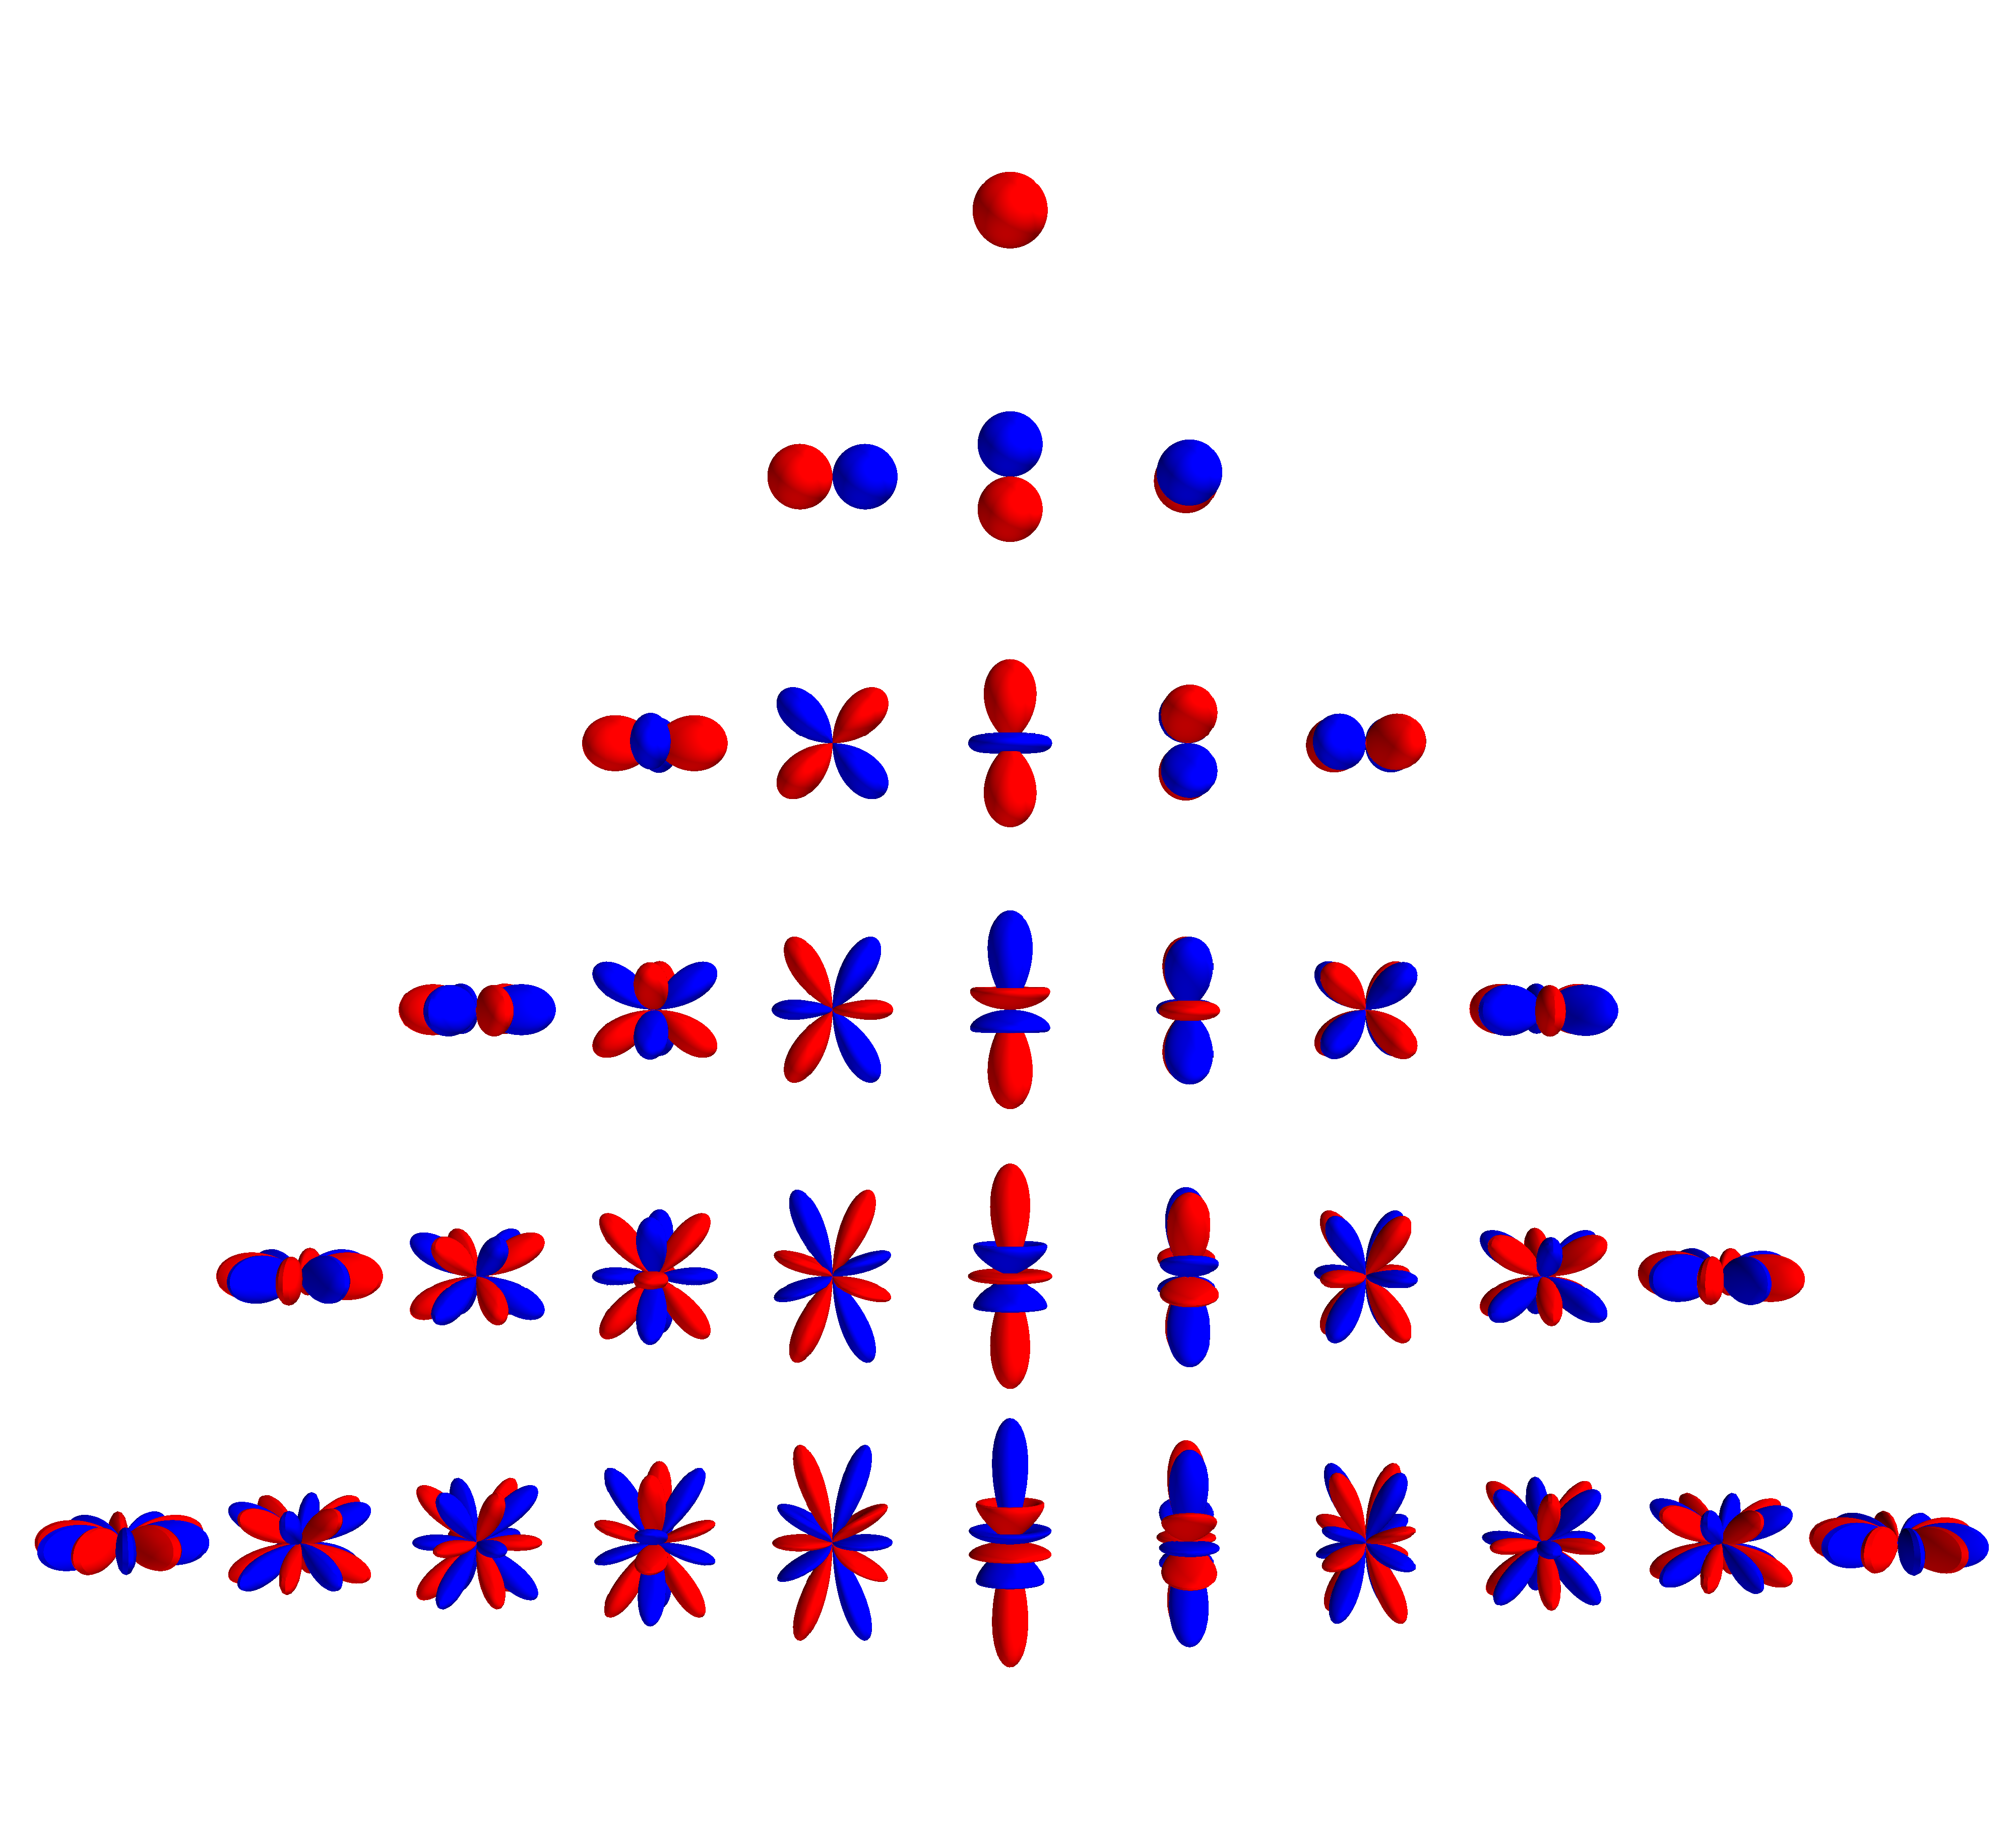
\includegraphics[width=\textwidth, interpolate=true, trim={0em 8em 0em 0em}]{figs/sph_harm}
  \vspace{-30pt}
  \caption{The spherical harmonic functions form an orthonormal basis for functions on the sphere. Red = positive, blue = negative.} 
  \label{fig:sph1}
\end{minipage}%
\hspace{0.75em}
\begin{minipage}{.45\textwidth}
  \centering
  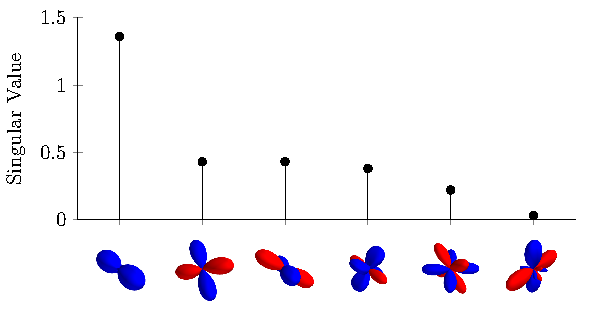
\includegraphics[width=\textwidth, interpolate=true]{figs/svs_dispim}
  \captionof{figure}{The angular singular value spectrum of a polarized
    dual-view selective plane microscope. In the same way that the modulation
    transfer function (MTF) characterizes the ability of an imaging system to
    transfer spatial harmonics, the angular singular value spectrum measures the
    ability of an imaging system to transfer spherical harmonics.}
  \label{fig:sph2}
\end{minipage}
\end{figure}

\noindent\textbf{Expected outcome:} A set of software tools that can be used
to reconstruct, visualize, and understand fluorophore orientations from data
collected by a wide class of polarized multiview microscopes.

\noindent\textbf{Potential complications:} We anticipate computationally
expensive reconstructions and visualizations as we refine our pipeline with
increasingly realistic physical models. We plan to employ graphical processing
units (GPUs) and cluster computing to ease the burden.

\noindent\textbf{Aim 2:} Demonstrate and verify three-dimensional fluorescence
orientation microscopy using a dual-view selective plane microscope and a
light-field microscope.

\noindent\textbf{Methods:} To demonstrate the dual-view selective plane
microscope we will use the dual inverted selective-plane illumination
microscope (diSPIM) platform developed by collaborators at the National
Institutes of Health (NIH). Prototype systems are available at the NIH and the
Marine Biological Laboratory (MBL). To demonstrate the light-field microscope we
will use a prototype system that is available at the MBL.

To verify our systems we will use several specimens with a known coupling
between fluorophore position and orientation. We are currently evaluating
several samples for this purpose---PBT
[poly(1,4-phenylene-2,6-benzo-bis-thiazole)] film, giant unilamellar vesicles
\cite{schmid}, and actin networks.

\noindent\textbf{Expected outcomes:} Clear evidence that our microscopes and
reconstruction techniques can reconstruct the position and orientation of
fluorophores. We will verify the position and orientation of fluorophores in a
sample using existing two-dimensional techniques, and we will verify our
three-dimensional techniques using this sample.

\noindent\textbf{Potential complications:} We expect initial disagreement
between our results and our known samples due to our use of simplified linear
models. We expect to be able to explain these discrepancies, and we plan to
refine our models if it is computationally feasible.

\noindent\textbf{Aim 3:} Demonstrate the value of three-dimensional fluorescence
  orientation microscopy for live-cell imaging.

\noindent\textbf{Methods:} We will collaborate with biologists at the Marine
Biological Laboratory to find applications for our techniques. We have already
identified several promising areas where the orientation of fluorophores in
three dimensions could report useful information:
\begin{itemize}
\item Cellular migration---the dynamics of actin networks responsible for
  cellular migration have been successfully studied with two-dimensional
  fluorescence orientation microscopy \cite{mehta2016}. We expect that more
  conclusions can be drawn using three-dimensional techniques.
\item Cellular transport---motor protein dynamics have been studied extensively
  using single-molecule techniques \cite{toprak2006}. Our proposed techniques
  may be able to improve on existing measurements.
\item Protein-protein interactions---fluorescence resonance energy transfer
  (FRET) is a widely used technique for measuring nanometer-scale distances
  between proteins. Most FRET experiments make assumptions about the relative
  orientation of the fluorophores involved \cite{nov2006}, and we expect that the
  proposed techniques could address these assumptions and improve the technique.
\end{itemize}

\noindent\textbf{Expected outcomes:} A biological research application for
three-dimensional fluorescence orientation microscopy. 

\noindent\textbf{Potential complications:} This aim depends on the previous two
aims, and it requires a collaboration with a to-be-identified biologist. With
our preliminary results in hand, we plan to start searching for a biological
collaborator soon. During the summer the MBL acts as a hub for biologists and
microscopists to test new techniques, so we expect to find a well-defined
biological application in coming months.

\noindent\textbf{Timeline:}
\begin{table}[H]
%  \hspace{-1em}
\begin{ganttchart}[%Specs
     y unit title=0.5cm,
     y unit chart=0.5cm,
     vgrid,hgrid,
     title height=1,
     title label font=\bfseries\small,
     bar/.style={fill=gray},
     bar height=0.4,
     group left shift=0,
     group right shift=0,
     group top shift=0.2,
     group height=.4,
     group peaks width={0.1},
     group peaks tip position={0},
     group peaks height={0.1},     
     inline]{1}{24}
    \gantttitle[]{2018}{9}
    \gantttitle[]{2019}{12} 
    \gantttitle[]{2020}{3} \\
    
    \gantttitle{Q2}{3}
    \gantttitle{Q3}{3}
    \gantttitle{Q4}{3}
    \gantttitle{Q1}{3}
    \gantttitle{Q2}{3}
    \gantttitle{Q3}{3} 
    \gantttitle{Q4}{3}
    \gantttitle{Q1}{3}\\

    \ganttgroup[inline=false]{Aim 1: Reconstruction pipeline}{1}{18}\\ 
    \ganttbar[inline=false]{Light-sheet reconstructions}{1}{3}\\
    \ganttbar[inline=false]{Visualization}{1}{6}\\
    \ganttbar[inline=false]{Light-field reconstructions}{4}{9}\\
    \ganttbar[inline=false]{Refine our techniques}{7}{18} \\

    \ganttgroup[inline=false]{Aim 2: Experimental verification}{1}{18} \\
    \ganttbar[inline=false]{Identify test specimens}{1}{3} \\
    \ganttbar[inline=false]{Verify light-sheet microscope}{1}{6} \\
    \ganttbar[inline=false]{Verify light-field microscope}{4}{9} \\
    \ganttbar[inline=false]{Verify refinements}{7}{18} \\

    \ganttgroup[inline=false]{Aim 3: Live-cell demonstration}{4}{21} \\ 
    \ganttbar[inline=false]{Identify research question}{4}{12} \\
    \ganttbar[inline=false]{Investigate research question}{10}{21} \\
    \ganttbar[inline=false]{\textbf{Thesis}}{22}{24}
  \end{ganttchart}
  \caption{Proposed project timeline.}
  \end{table}

\section*{References}
\setlength\biblabelsep{0.01\textwidth}
\printbibliography[heading=none]

\end{document}